% F091｜完全立方数的立方根尾数速判｜04_examples.tex
% 继承上传模板的 LaTeX 环境；当前条目的内容独立编写。
\clearpage
\begin{examplebox}
\textbf{\textcolor{CExample}{例 1：口算立方根1728}}
\par\medskip
\begin{center}
% F091｜split 原创简明教学示意图
\begin{tikzpicture}[>=stealth,scale=.9]
\node[draw,rounded corners,fill=teal!9,minimum width=2.5cm,minimum height=1.25cm] (a) at (0,0){$\underbrace{103}_{\text{高位}}\mid\underbrace{823}_{\text{低位}}$};
\node[draw,rounded corners,fill=orange!9,minimum width=3.2cm,minimum height=1.25cm] (b) at (4.5,0){$4^3\le103<5^3$};
\node[draw,rounded corners,fill=teal!15,minimum width=2.3cm,minimum height=1.25cm] (c) at (9.0,0){$\sqrt[3]{103823}=47$};
\draw[->,thick] (a)--(b);\draw[->,thick] (b)--(c);
\node at (4.5,-1.2){\small 高位定十位，末位定个位};
\end{tikzpicture}

\end{center}
\medskip
写作 $1\mid728$。左侧 $1$ 满足 $1^3\le1<2^3$，所以十位 $1$；个位 $8$ 对应 $2^3$，所以个位 $2$。得 $\boxed{12}$；核验 $12^3=1728$。
\end{examplebox}
\clearpage
\begin{examplebox}
\textbf{\textcolor{CExample}{例 2：口算立方根2197}}
\par\medskip
\begin{center}
% F091｜last 原创简明教学示意图
\begin{tikzpicture}[>=stealth,scale=.89]
\node[draw,rounded corners,fill=teal!9,minimum width=3cm] (a) at (0,0){$7^3=343$};
\node[draw,rounded corners,fill=orange!9,minimum width=3cm] (b) at (4.1,0){尾数 $3$};
\node[draw,rounded corners,fill=teal!15,minimum width=3cm] (c) at (8.2,0){根的个位 $7$};
\draw[->,thick] (a)--(b);\draw[->,thick] (b)--(c);
\end{tikzpicture}

\end{center}
\medskip
写作 $2\mid197$，左侧 $1^3\le2<2^3$，十位 $1$；个位 $7$ 只由 $3^3$ 得到，所以根为 $\boxed{13}$。
\end{examplebox}
\clearpage
\begin{examplebox}
\textbf{\textcolor{CExample}{例 3：口算立方根103823}}
\par\medskip
\begin{center}
% F091｜verify 原创简明教学示意图
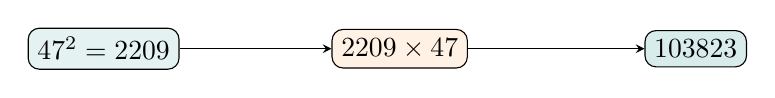
\begin{tikzpicture}[>=stealth,scale=.94]
\node[draw,fill=teal!10,rounded corners] (a) at (0,0){$47^2=2209$};
\node[draw,fill=orange!10,rounded corners] (b) at (4,0){$2209\times47$};
\node[draw,fill=teal!15,rounded corners] (c) at (8,0){$103823$};
\draw[->] (a)--(b);\draw[->] (b)--(c);
\end{tikzpicture}

\end{center}
\medskip
写作 $103\mid823$，有 $4^3=64\le103<5^3=125$，十位 $4$；末位 $3$ 对应个位 $7$，得到 $\boxed{47}$。最后验算 $47^3=103823$。
\end{examplebox}
